\documentclass[11pt]{article}

\usepackage[margin=1in]{geometry}
\usepackage{amsmath}
\usepackage{graphicx}
\usepackage{float}

\title{RL Lab 2 -- Dynamic Programming}
\author{Fotios Kapotos}
\date{}

\begin{document}

\maketitle

\section{Policy evaluation}


The value function increases with the state index, indicating that higher states yield larger expected long-term returns under the evaluated policy. The smooth and monotonic profile suggests that the in-place Bellman updates have converged properly to $v_{\pi}$. The slight decrease at the final state reflects a boundary or terminal effect, where fewer future rewards can be accumulated.

The action--state heatmap shows that the policy is deterministic, assigning probability 1 to a single action for all states and 0 to the others. Hence, the evaluated pricing scheme is stationary and non-stochastic. The resulting value function therefore represents the expected return when consistently applying this single action in every state.


\begin{figure}[h]
    \centering
    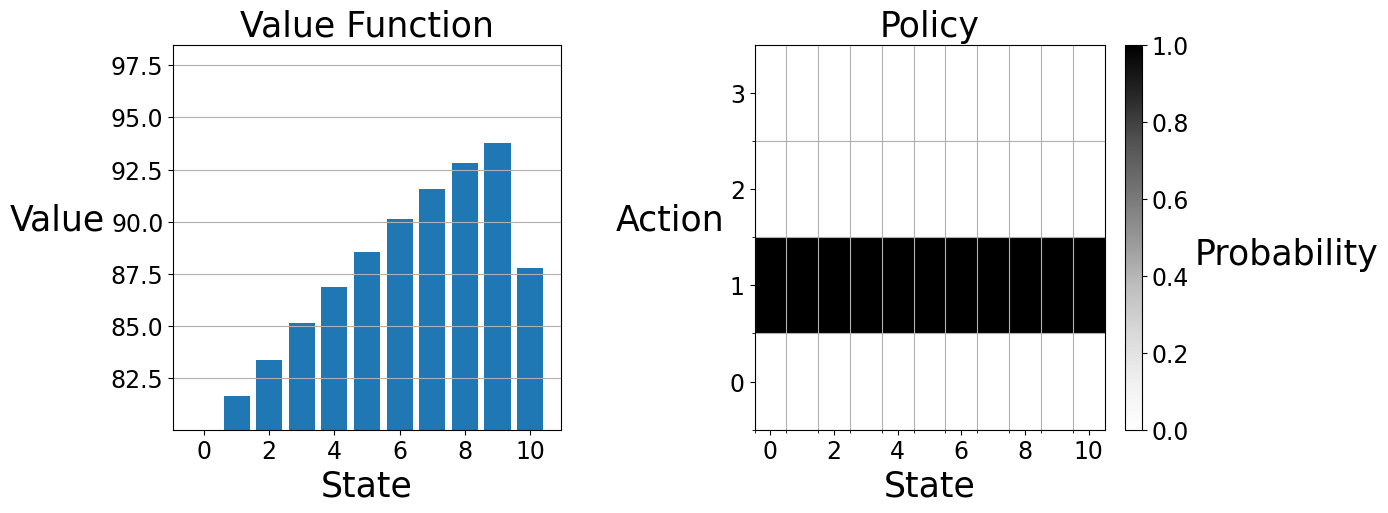
\includegraphics[width=0.85\linewidth]{../figures/policy_eval.png}
    \caption{}
\end{figure}

\section{Policy iteration}


Policy iteration converges to a state-dependent deterministic policy. Unlike the initial policy evaluation result (Section 1), where the same action was selected for all states, the improved policy now differentiates between low and high states.

From the heatmap, lower states select one pricing action (action 0), while the highest states switch to a different action (action 3). This indicates that the greedy improvement step successfully adapted prices depending on occupancy level. Intuitively, when many parking spaces are available (low state index), a lower price maximizes long-term occupancy and revenue, whereas when the parking lot is nearly full (high state index), a higher price becomes optimal.

The corresponding value function increases smoothly with the state and reaches higher values than in Section 1, confirming that policy iteration has produced a strictly more efficient policy. The change in action near the highest states reflects the trade-off between immediate revenue and future discounted returns captured by the Bellman optimality principle.

\begin{figure}[h]
    \centering
    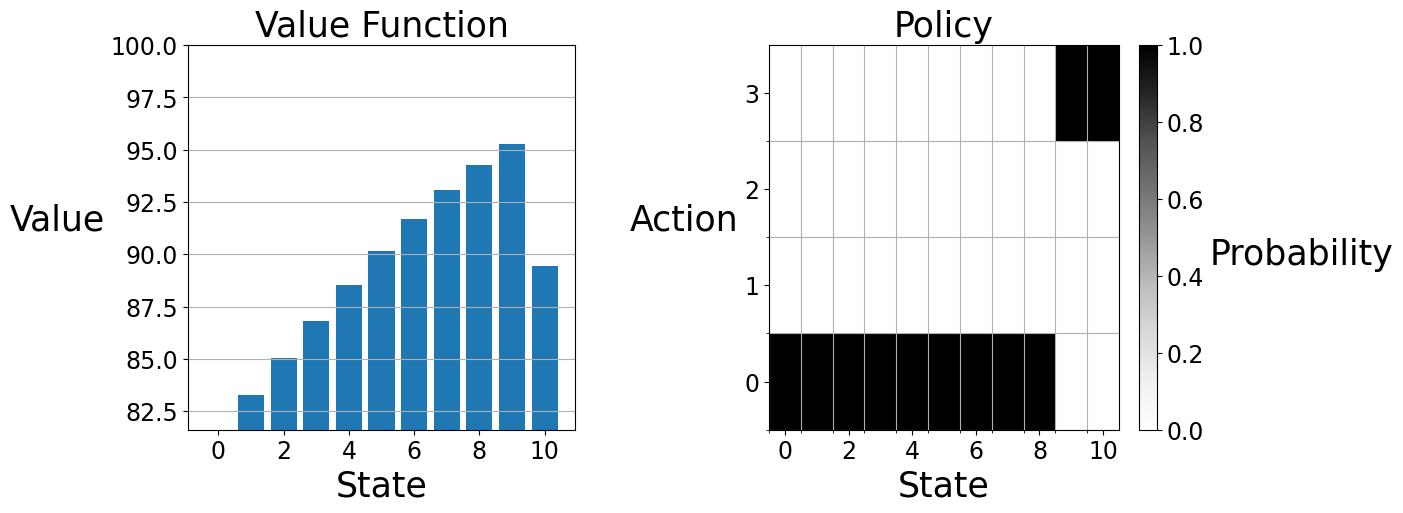
\includegraphics[width=0.85\linewidth]{../figures/policy_iter.png}
\end{figure}

\section{Value iteration}

Value iteration directly applies the Bellman optimality update and converges to the optimal value function $v_*$. The resulting value profile is increasing in the state, with a slight drop at the boundary state due to limited future rewards. The shape closely matches that obtained via policy iteration, confirming convergence to the same optimal solution.

The derived policy is deterministic and state-dependent. Lower states select a lower pricing action, while the highest states switch to a higher price. This threshold structure reflects the optimal trade-off between immediate revenue and future discounted returns. The agreement between value iteration and policy iteration validates the correctness of both implementations and confirms that the optimal pricing strategy has been recovered.

\begin{figure}[h]
    \centering
    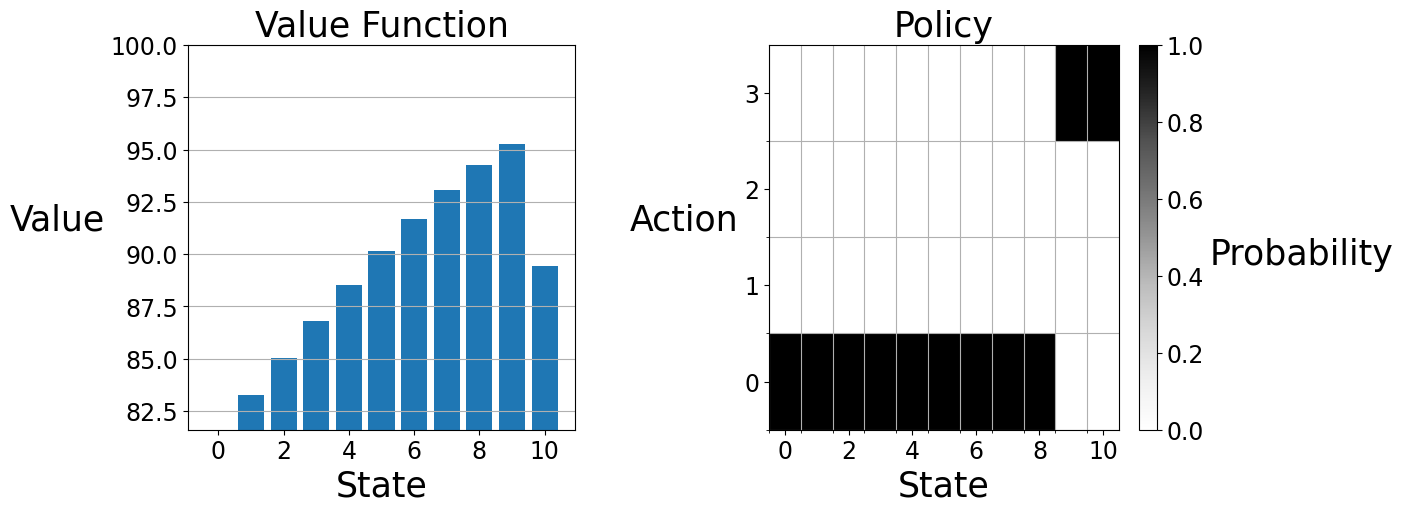
\includegraphics[width=0.85\linewidth]{../figures/value_iter.png}
\end{figure}

\end{document}